\section{RESULTADOS}


\subsection{Invasibilidad}
Dada la parametrizaci\'on usada y asumiendo :
\begin{enumerate}
\item $\beta_R = \beta_C = \beta_P = \beta$
\end{enumerate}

Derivamos expl\'icitamente las siguientes condiciones para cada criterio de invasibilidad \textbf{I} y zona \textbf{Z(I)} asociada a \textbf{I} en funci\'on a $k_{\RC},k_{\CP}$ y $m_P$.

\subsubsection{C $\to$ R}

\begin{equation}
  \frac{dC}{dt} >0 \iff  m_P^{h_R +1 - 2\beta} > \zeta_1(k_{\RC},k_{\CP}) = k_{\CP}^{2\beta -1 -h_R}(\frac{\chi_1}{\chi_0})
\end{equation}
Donde:
\begin{equation}
  \begin{aligned}
    h_R &= p_v + 2(D_R - 1)p_d \\
    \chi_0 &= \varepsilon_1 \kappa_0\alpha_{0,1} g(k_{\RC}) \\
    g(k_\RC) &= f_1(k_{\RC})k_{\RC}^{1-\beta}\\
    \chi_1 &= q_{0,1} 
  \end{aligned}
\end{equation}
Entonces:
\begin{equation}
\mathbf{Z(I_{\C\to \R})} := \{ (k_{\RC},k_{\CP},m_P) \in \mathbb{R}^3_+ / m_p^{h_R + 1 - 2\beta} > \zeta_1(k_{\RC},k_{\CP}) \}
\end{equation}


Dada la relaci\'on anterior, podemos deducir la influencia de los par\'ametros del modelo sobre la invasibilidad de $C$.\\

En particular dado que $f_1(k_{\RC}) \to 0 (k_{\RC} \to 0)$ y $\beta <1$ tenemos que $\chi_0 \to 0 (k_{\RC} \to 0)$,para un valor acotado de $\kappa_0$,y por lo tanto valores extremadamente peque\~nos de $k_{\RC}$ siempre ser\'an exclu\'idos de $\mathbf{Z(I_{\C\to \R})}$ si mantenemos $m_P$ y $k_{\CP}$ constante(un comportamiento an\'alogo se observa para $k_\CP$ peque\~nos), dicho esto al aumentar $k_{\CP}$, $\kappa_0$ y $m_P$ el m\'inimo $k_{\RC}$ disminuye, asu ves dado que el impacto de $m_P y k_\CP$ esta influenciado por la dimensi\'on del espacio de b\'usqueda esta disminuci\'on es mas fuerte para ambientes $3D$.\\

Para valores fijos de $k_{\CP}, \kappa_0 ,m_P$,el valor m\'aximo de $k_{\RC}$ en $\mathbf{Z(I_{\C\to \R})}$ depender\'a del valor de $\phi$ y $fm$. Sin embargo para los distintos $fm$ tenemos un comportamiento cualitativo similar , debido a la similitud existente entre $f_1$ para distintos $fm$(v\'ease anexos). Dado la similitud entre $g$ y $f_1$ por un tratamiento similar al descrito en anexos podemos observar que para $\phi$ \emph{suficientemente peque\~no} $\chi_0$ crece mon\'otonamente con respecto a $k_\RC$ por lo tanto se observa la presencia de un valor umbral $k$ tal que por encima de \'el la invasi\'on de $C$ es posible. A su vez para valores de $\phi$ \emph{suficientemente grandes} tenemos que $\chi_0$ presenta un valor m\'aximo por encima del cual decrece mon\'otonamente, es m\'as $\chi_0 \approx c k_{RC}^{h - \phi}$ para valores de $k_\RC$ elevados(donde $h$ depende de $fm$) y por tanto estos ser\'ian exclu\'idos de $\mathbf{Z(I_{\C\to \R})}$ dado que al mantener $m_P$ y $k_\CP$ fijos cambios en $k_\RC$ simplemente indican cambios en la masa de $m_R$ podemos interpretar estos resultados de la siguiente manera, sin importar $\phi$, $m_R$ tiene que tener un tama\~no m\'inimo el cual permita a $C$ invadir, esto debido al hecho que $m_R$ influencia la capacidad de carga de $R$, y por ende la energ\'ia disponible a $C$ al momento de la invasi\'on, sin embargo valores elevados de $m_R$ son inviables para $C$ para $\phi$ \emph{suficientemente grandes} ya que en estos casos a pesar de que el sistema presenta una gran cantidad de energ\'ia disponible, debido a la baja probabilidad de captura de $R$ por parte de $C$ no se traducen en aumentos en biomasa de $C$, es decir lo importante para $C$ al momento de la invasi\'on no solamente es la energ\'ia total presente en el sistema sino que \'esta se encuentre en una \emph{forma} que pueda ser explotada por $C$.\\


Si mantenemos $\kappa_0,k_\CP$ y $k_\RP$ fijos, observamos que para que sea posible la invasi\'on de $C$, $m_P$ tiene que superar un valor dado. Dado que aumentos en $m_P$ para size ratios fijos implican aumentos en las masas de $R$ y $C$ respectivamente, esto nos dice que existe un tama\~no de $C$ y$R$ por encima del cual la invasi\'on de $C$ es posible.
La dimensi\'on del espacio de b\'usqueda afecta positivamente a $\chi_0$(si asociamos cambios en $\kappa_0$, y con $k_\RC > 10^{-30}$), sin embargo debido a que aumenta $h$ su impacto total sobre la invasibilidad puede ser negativo para valores elevados de $k_\RC$(i.e cuando el m\'inimo $k_\RC$ necesario para la invasi\'on es elevado, como se da para $k_\CP$ y $m_P$ peque\~nos), siendo m\'as precisos siempre que $\frac{\chi_1}{\chi_0} >1$ en ambientes $2D$ tenemos que el impacto es positivo, pero para $\frac{\chi_1}{\chi_0} < 1$ el impacto es negativo si $ (\frac{\chi_1}{\chi_0})_{3D}^\frac{1 + h_{2D} - 2 \beta}{1 + h_{3D} - 2 \beta} >  (\frac{\chi_1}{\chi_0})_{2D} $.\\


\begin{figure}
  \centering
  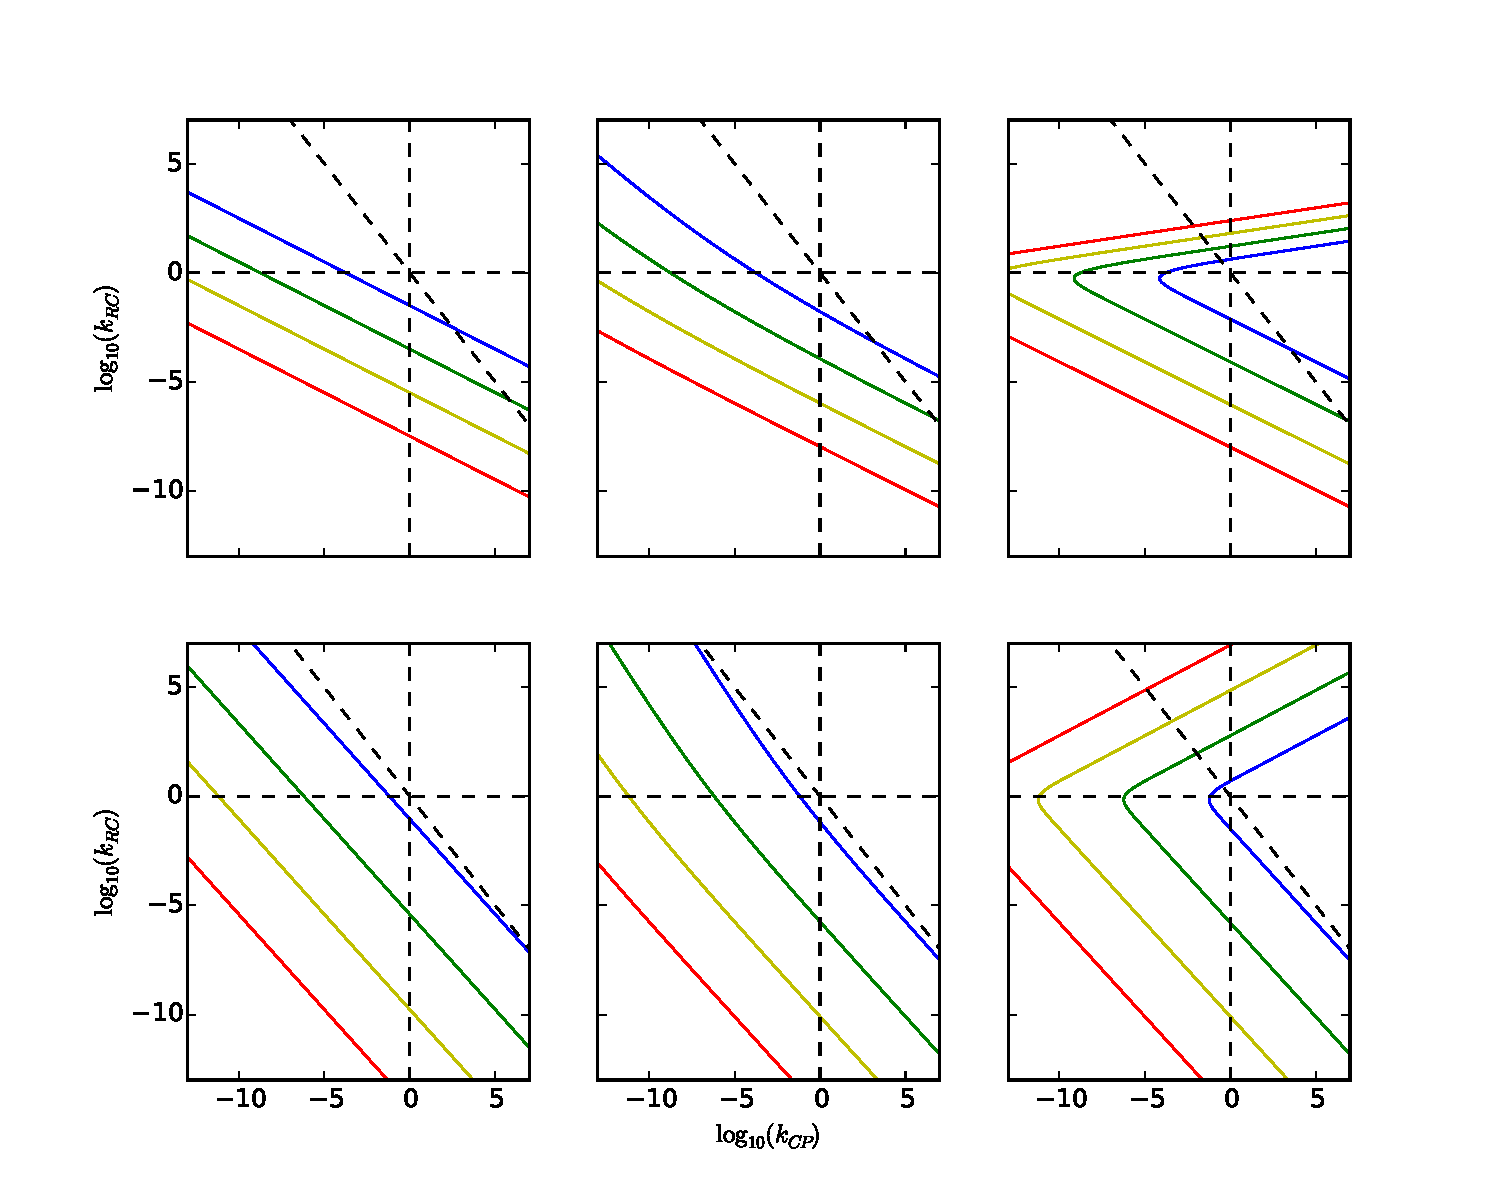
\includegraphics[width = 0.99\textwidth]{./Plots/Z(IC2)AcGrGr.pdf}
  \caption[Env $Z(IC2)$]{\emph{Envolturas de Invasibilidad} para el caso de el depredador intermedio $C$ como invasor frente a una comunidad receptora formada por $R$. La fila superior es para espacios de b\'usqueda bidimensionales y la inferior tridimensionales, las columnas de izquierda a derecha aumentan el valor de $\phi$, siendo $0.02,0.2$ y $2$ respectivamente.Las diferentes lineas implican distintas masas de depredador $m_P$ :({\hwplotR}) $10^5 kg$,  ({\hwplotY}) $1kg$, ({\hwplotG}) $10^{-5}kg$ y ({\hwplotB}) para $10^{-10}kg$. ({\hwplotK}) separa las zonas donde $K_{RC},K_{CP},k_{RP}$ son mayores o menores que 1 respectivamente. $k_0 = 0.1$ y $k_0 = 30$ para el caso $2D$ y $3D$ respectivamente, los valores de los otros par\'ametros son los descritos en el anexo \ref{subsec:params}}
  \label{fig:Z(IC2)}
\end{figure}

\subsubsection{P $\to$ R}

\begin{equation}
  \frac{dP}{dt} >0 \iff  m_P > \zeta_2(k_{\RC},k_{\CP}) = (\frac{q_{0,2}}{\eta_0})^{\frac{1}{h_R +1 - 2\beta}}
\end{equation}
Donde:
\begin{equation}
  \begin{aligned}
    \eta_0 &= \varepsilon_2 \kappa_0\alpha_{0,2} f_2(k_{\RP})k_{\RP}^{1-\beta} \\
  \end{aligned}
\end{equation}

\begin{equation}
\mathbf{Z(I_{\PP \to \R})} := \{ (k_{\RC},k_{\CP},m_P) \in \mathbb{R}^3_+ / m_p > \zeta_2(k_{\RC},k_{\CP}) \}
\end{equation}

El comportamiento es similar al descrito anteriormente, reemplazando $k_\RC$ por $k_\RP$ en nuestra discusi\'on anterior.


\begin{figure}
  \centering
  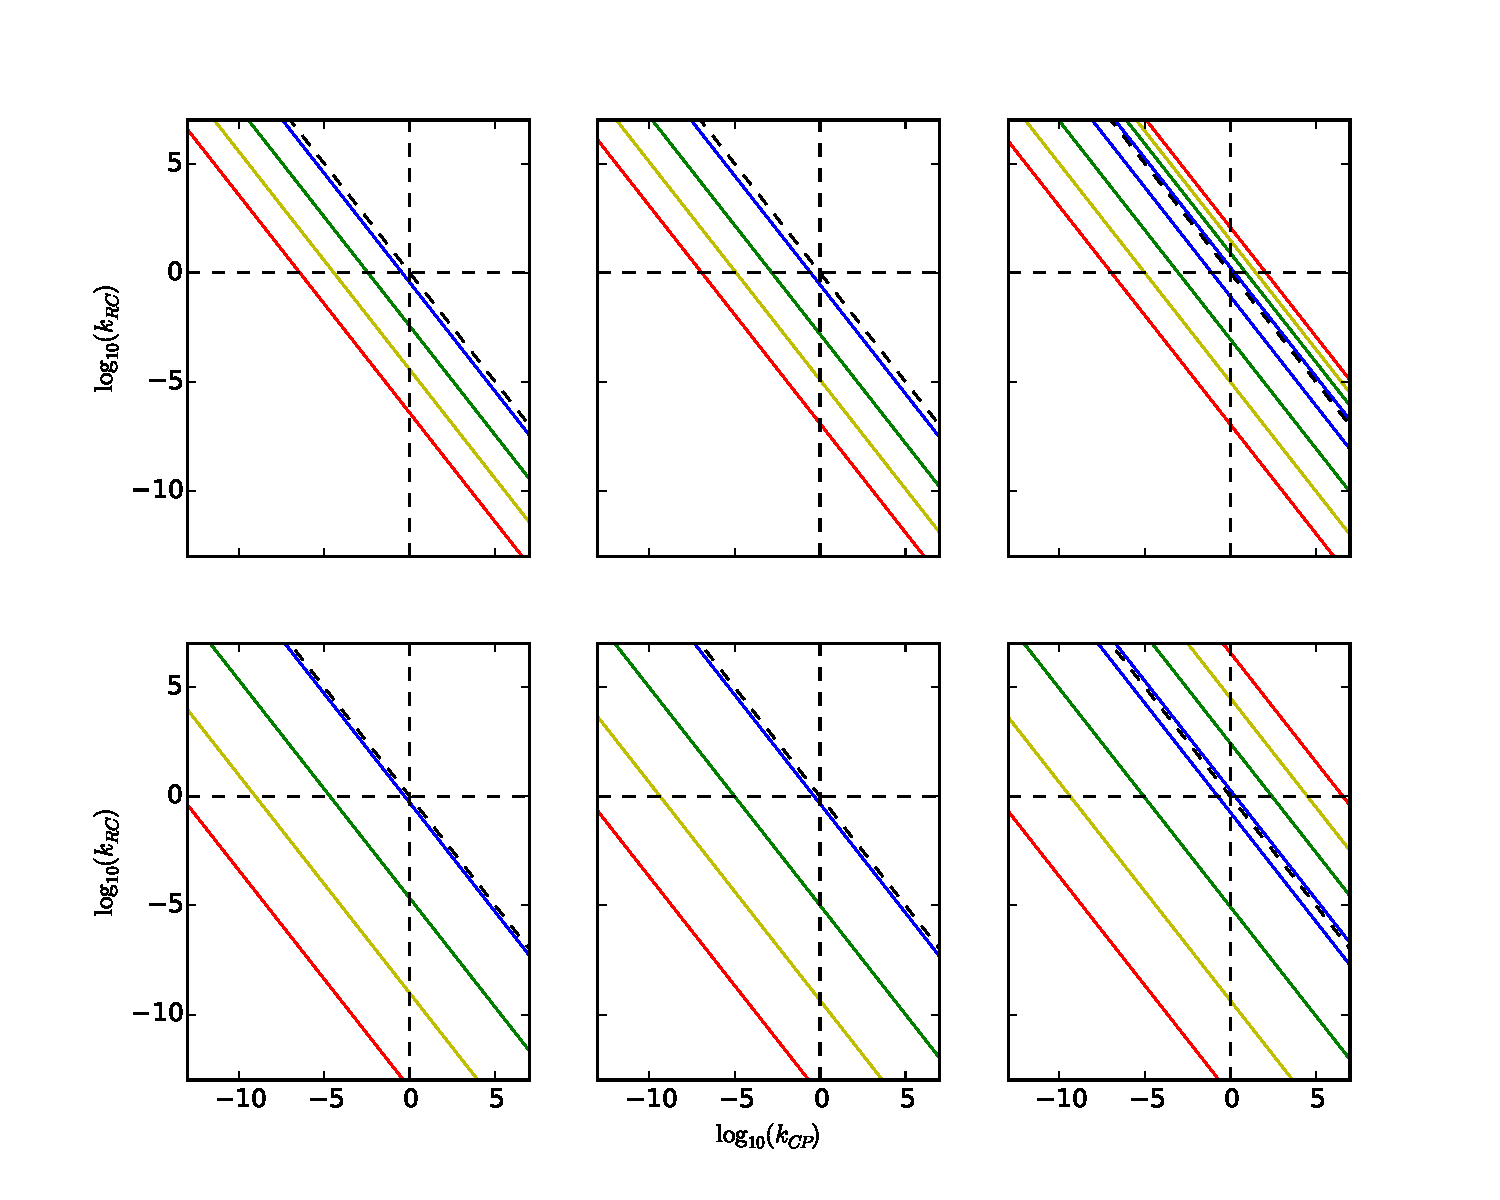
\includegraphics[width = 0.99\textwidth]{./Plots/Z(IC3)AcGrGr.pdf}
  \caption[Env $Z(IC2)$]{\emph{Envolturas de Invasibilidad} para el caso de el depredador intermedio $P$ como invasor frente a una comunidad receptora formada por $R$.Las dem\'as especificaciones se comparten con la figura ~\ref{fig:Z(IC2)}}
  \label{fig:Z(IC3)}
\end{figure}


Asumiendo a su vez que $D_R = D_C = D$

Definamos:
\begin{equation}
  h = p_v + 2(D-1)p_d
\end{equation}

\subsubsection{P $\to$ C-R}
\begin{equation}
  \frac{dP}{dt}  >0 \iff m_P > \zeta_3(k_{\RC},k_{\CP}) = (\frac{\xi_4\xi_2}{\xi_3 + \xi_4 - q_{0,2}})^{\frac{1}{h + 1 - 2\beta}}
\end{equation}

Donde:
\begin{equation}
  \begin{aligned}
    \xi_0 &= \frac{q_{0,1} k_{\CP}^{\beta - h}}{\epsilon_1 \alpha_{0,1} f_1(k_{\RC})}\\
    \xi_1 &= \frac{r_0 k_{\CP}^{\beta-h}}{\alpha_{0,1} f_1(k_{\RC})k_{\RC}^{1-\beta}}\\
    \xi_2 &= \frac{\xi_0}{k_0 k_{\RP}^{1-\beta}} \\
    \xi_3 &= \varepsilon_2 \alpha_{0,2} f_2(k_{\RP}) \xi_0\\
    \xi_4 &=\varepsilon_3 \alpha_{0,3} f_3(k_{\CP}) \xi_1
  \end{aligned}
\end{equation}

Por lo tanto 
\begin{equation}
\mathbf{Z(I_{\PP \to \C-\R})} := \{ (k_{\RC},k_{\CP},m_P) \in \mathbb{R}^3_+ / m_p > \max\{\zeta_1(k_{\RC},k_{\CP}),\zeta_3(k_{\RC},k_{\CP})\} \}
\end{equation}

A diferencia de los dos casos anteriores la complejidad de esta expresi\'on imposibilita un an\'alisis a la misma profundidad que el descrito anteriormente, y simplemente nos referimos a ciertos casos particulares.\\
En primer lugar esta relaci\'on solo es posible si :
\begin{equation}
  \xi_3 + \xi_4 > q_{2,0}
\end{equation}

Por lo que nos centramos primero a evaluar la influencia de $k_\RC$ y $k_\CP$ sobre esta condici\'on, dado que $\xi_3$ esta relacionado con la tasa de consumci\'on del recurso basal y $\xi_4$ con la tasa m\'axima de consumci\'on sobre el consumidor intermedio(i.e la tasa de consumci\'on a la m\'axima abundancia para $C$) esta relaci\'on concuerda con la intuici\'on de la existencia de un nivel de energ\'ia m\'inimo para la invasi\'on de $P$.Reescribi\'endola tenemos:
\begin{equation}
  \frac{k_{\CP}^{\beta - h}}{f_1(k_\RC)}(a_0 f_2(k_\RP) + q_1 \frac{f_3(k_\CP)}{k_\RC^{1-\beta}}) > q_{2,0}
\end{equation}
De donde dependiendo del valor de $\phi$ y $fm$ podemos tener comportamientos distintos, en particular para $f_1, f_2$ crecientes esta relaci\'on no se cumplir\'ia para $k_\RC$ suficientemente grande debido a su influencia negativa sobre $\xi_4$ 







Asumiendo que los valores de $k_\RC , k_\CP , m_P$ son tales que es posible la invasi\'on de $C$(es decir todas las restricciones descritas para la invasibilidad de $C$ ya se aplican, en particular $\kappa_0$ afecta positivamente el cumplimiento de esta condici\'on), reescribiendo la condici\'on anterior observamos que $\xi_2$ es justamente $\zeta_1(k_{\RC},k_{\CP})$ y por ende tenemos que $m_P^{1 + h - 2\beta} > \xi_2$ , y en este caso tendr\'iamos que la condic\'on se seguir\'ia cumpliendo siempre que $\frac{\xi_4}{\xi_3 + \xi_4 - q_{0,2}} \leq 1$ y una condici\'on necesaria para que no se cumpla es $\frac{\xi_4}{\xi_3 + \xi_4 - q_{0,2}} > 1$ por lo tanto nos enfocamos en analizar las condiciones para las que $ \xi_3 < q_{0,2}$ esto es:
\begin{equation}
  \frac{f_2(k_\RP) k_\CP^{\beta - h}}{f_1(k_\RC)} < \frac{q_{0,2} \varepsilon_1 \alpha_{0,1}}{q_{0,1} \varepsilon_2 \alpha_{0,2}}
\end{equation}

De esta relaci\'on podemos inferir la influencia de $k_\RC$ y $k_\CP$ sobre el criterio, de la siguiente manera:\\
Para un $k_\RC$ fijo , $k_\CP$ afecta $g_2 := f_2(k_\RP) k_\CP^{\beta -h}$  de modo similar a como $k_\RC$ afectaba $g$ en el caso de la invasi\'on de $C$, es decir para valores de $\phi$ suficientemente peque\~nos $g_2$ tiende a crecer con $k_\CP$ lo que imposibilitar\'ia el cumplimiento de la condici\'on anterior para valores elevados de $k_\CP$ y por ende ser\'ia posible la invasi\'on de $P$. Sin embargo para valores de $\phi$ suficientemente grandes(condicionados a $fm$), $g_2$ tiende a 0 para valores elevados de $k_\CP$ y por lo tanto podr\'iamos esperar que $P$ no pueda invadir a $C-R$ para valores de $k_\CP$ suficientemente grandes(No discutimos el comportamiento a valores peque\~nos de $k_\CP$, debido a que estos se consideran en las condiciones para la invasibilidad de $C$).\\
El efecto de $k_\RC$ es mas d\'ificil de discernir y lo ejemplificamos asumiendo que $fm = Grazing$ tanto para $f_1$ como para $f_2$, en este caso tenemos:
\begin{equation}
  \frac{(1 + k_\RC^\phi) k_\CP^{(D-1)p_d + \beta - h}}{1+(k_\RC k_\CP)^\phi} <\frac{q_{0,2} \varepsilon_1 \alpha_{0,1}}{q_{0,1} \varepsilon_2 \alpha_{0,2}}
\end{equation}




En todos los casos explorados $Z(I_{\PP \to \R - \C})$ tiende a crecer con respecto a aumentos en la masa del depredador $m_P$, y adem\'as forman una secuencia encajante, igual que en los casos anteriores se observa una respuesta cualitativa similar en cambios respecto a $m_p$ y $k_0$. Sin embargo el crecimiento no es uniforme, las zonas relativas si bien tienden a crecer lo hacen de manera desigual dependiendo adem\'as del valor del par\'ametro $\phi$.\\

El valor de $\phi$ controla en cierta la ``forma'' de $Z(I_{\PP \to \R - \C})$, observandose por lo general una relaci\'on inversa del valor de $phi$ y el \'area total de $Z(I_{\PP \to \R - \C})$ irrespectivamente de la masa. Sin embargo afecta de manera desigual los distintos tipos de Comunidades.\\ Por ejemplo, en el caso de comunidades con distribuci\'on de masa $C_1$ el par\'ametro es pr\'acticamente irrelavante sobre la zona relativa $Z(I_{\PP \to \R - \C})_1$, y por el contrario para comunidades $C_5$ el cambio es dram\'atico, dado que entre $\phi  = 0.02 - 2$, $Z(I_{\PP \to \R - \C})_5$ pasa de ser no vac\'ia y cubrir en su totalidad(en el caso $3D$) a $C_5$ (i.e $Z(I_{\PP \to \R - \C})_5 = C_5$) para todas las masas $m_P$ exploradas, a ser vac\'io para todo $m_P$ en el segundo caso.\\
La dimensi\'on del espacio de b\'usqueda afecta el \'area total y las \'areas relativas de $Z(I_{\PP \to \R - \C})$.\\
En el primer caso observamos que generalmente es mayor en espacios tridimensionales(3D) y esta diferencia se acent\'ua conforme la masa $m_P$ aumenta,en el segundo  tenemos un patr\'on muy similar pero en este caso para $m_P$ bajos se pueden observar comunidades donde el \'area de la zona relativa es mayor en ambientes bidimensionales, como por ejemplo $Z(IC_3)$ para $m_P = 10^{-10}$. \\
Algo que resaltar es que el borde inferior(en escala logar\'itmica) tiende a ser \emph{paralelo} a $(\log_{10}(K_{CP}),-log_{10}(K_{RC}))$ para espacios de b\'usqueda $3D$ y no en el caso $2D$


\begin{figure}
  \centering
  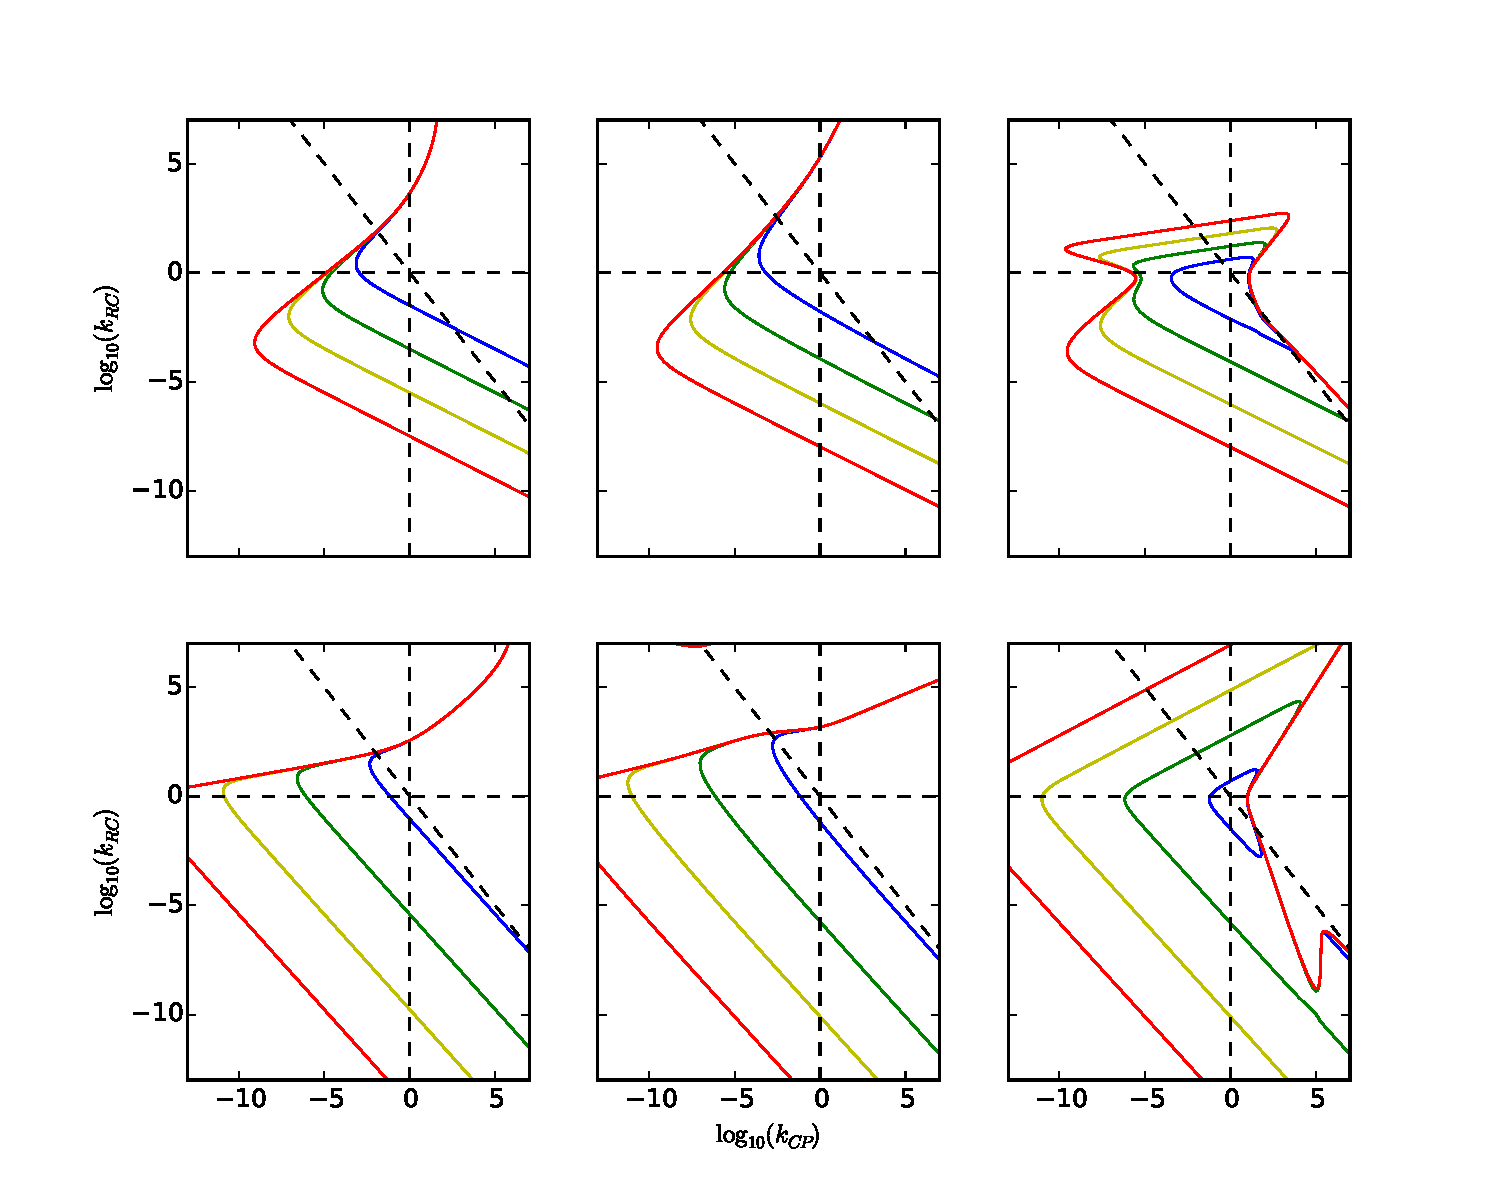
\includegraphics[width = 0.99\textwidth]{./Plots/Z(IC4)AcGrGr.pdf}
  \caption[Env $Z(IC4)$]{\emph{Envolturas de Invasibilidad} para el caso de el depredador tope $P$ como invasor frente a una comunidad receptora formada por $R-C$ .Las dem\'as especificaciones se comparten con la figura ~\ref{fig:Z(IC2)}}
  \label{fig:Z(IC4)}
\end{figure}


\subsubsection{C $\to$ P-R}
\begin{equation}
  \frac{dC}{dt}  >0 \iff m_P < \zeta_4(k_{\RC},k_{\CP}) = (\frac{\gamma_4\gamma_2}{\gamma_5 + \gamma_4 - \gamma_3})^{\frac{1}{h + 1 - 2\beta}}
\end{equation}

Donde:
\begin{equation}
  \begin{aligned}
    \gamma_0 &= \frac{q_{0,2}}{\varepsilon_2 \alpha_{0,2} f_2(k_{\RP})}\\
    \gamma_1 &= \frac{r_0 k_{\RP}^{\beta -1}}{\alpha_{0,2} f_2(k_{\RC})}\\
    \gamma_2 &= \frac{\gamma_0}{\kappa_0 k_{\RP}^{1-\beta}} \\
    \gamma_3 &= \varepsilon_1\alpha_{0,1} f_1(k_{\RP}) k_{\CP}^{h -1} \gamma_0\\
    \gamma_4 &=\alpha_{0,3} f_3(k_{\CP}) \gamma_1 \\
    \gamma_5 &= q_{0,1} k_{\CP}^{\beta-1}
  \end{aligned}
\end{equation}

Por lo tanto tenemos que:

\begin{equation}
\mathbf{Z(I_{\C \to \PP-\R})} := \{ (k_{\RC},k_{\CP},m_P) \in \mathbb{R}^3_+ / \zeta_4(k_{\RC},k_{\CP}) > m_p > \zeta_2(k_{\RC},k_{\CP}) \}
\end{equation}

Juntando ambas zonas anteriores tenemos que la region de \emph{invasibilidad mutua} $Z_{IM} := Z(I_{\C \to \PP-\R}) \cap Z(I_{\PP \to \C-\R})$ , resulta:


\begin{equation}
\mathbf{Z_{IM}} := \{ (k_{\RC},k_{\CP},m_P) \in \mathbb{R}^3_+ / \zeta_4(k_{\RC},k_{\CP}) > m_p > \max \{ \zeta_2(k_{\RC},k_{\CP}) , \zeta_1(k_{\RC},k_{\CP}) , \zeta_3(k_{\RC},k_{\CP}) \}
\end{equation}



Para una zona $Z$ en particular definimos la \emph{zona relativa} al tipo de comunidad $n$ como $Z_n = Z \cap C_n$. \\
A continuaci\'on se describen resultados para la combinaci\'on de estrategias de forrajeo \emph{Grazing-Grazing-Active}. Dado que en los otros dos casos se obtiene una respuesta cualitativa similar estos no ser\'an detallados.





\subsubsection{$C \to R-P$}
De forma similar al caso anterior tenemos que el \'area total de $Z(I_{\C \to \R - \PP})$ esta relacionada positivamente con el valor de $m_P$ y $k_0$, sin embargo a diferencia del caso anterior las zonas para distintos $m_P$ si bien tienen intersecci\'on no vac\'ia ,no estan incluidas una en otra. Es decir a parte de crecimiento tenemos un desplazamiento conforme aumenta $m_P$. \\

En este caso es bastante notoria la no uniformidad en el \'area de las zonas relativas.\\

El par\'ametro $\phi$ juega un papel importante en la topolog\'ia de $Z(I_{\C \to \R - \PP})$, para valores peque\~nos el conjunto es conexo, sin embargo para $\phi = 2$(y $m_p>10^{-10}$ y $k_0 > 3$ en el caso $3D$) el conjunto tiene 2 componentes $\vartheta_C^1$ y $\vartheta_C^2$ . La distancia entre estas componenes aumenta con $m_P$ y $k_0$ ; podemos distinguirlas por el hecho que una de ellas $\vartheta_C^1$ intersecta principalmente las zonas $C_3,C_4,C_5$ y la otra $\vartheta_C^2$ las zonas $C_1,C_2,C_6$, es decir se caracterizan por contener comunidades con $k_{\RP} >1 $($\vartheta_C^1$) o $k_{\RP}<1$ ($\vartheta_C^2$). Siendo la primera la que presenta mayor \'area. \\
Para $\phi = 0.2 ,0.02$  tenemos que $Z(I_{\C \to \R - \PP})$ intersecta principalmente a las zonas $C_2,C_3$(Comunidades con $k_{\RC}>1$ y$k_{\CP} <1$) y posee una ``\emph{cola}'' que es paralela(en escala logar\'itmica) a $\log_{10}(K_{CP}) = -log_{10}(K_{RC})$ y que dependiendo del valor de $m_P$($k_0$) esta contenido en las zonas $C_1,C_2,C_6$ o $C_3,C_4,C_5$, es decir $k_{RP} > 1$ o $k_{RP}<1$. \\

La dimensi\'on del espacio de b\'usqueda igual que en el caso anterior afecta el \'area total de $Z(I_{\C \to \R - \PP})$ la cual es mayor en ambientes tridimensionales.\\
Para $\phi = 2$ se observa que el \'area de $\vartheta_C^2$ es por lo general mayor en ambientes bidimensionales y lo contrario ocurre con el otro componente en ambientes 3D.

\begin{figure}
  \centering
  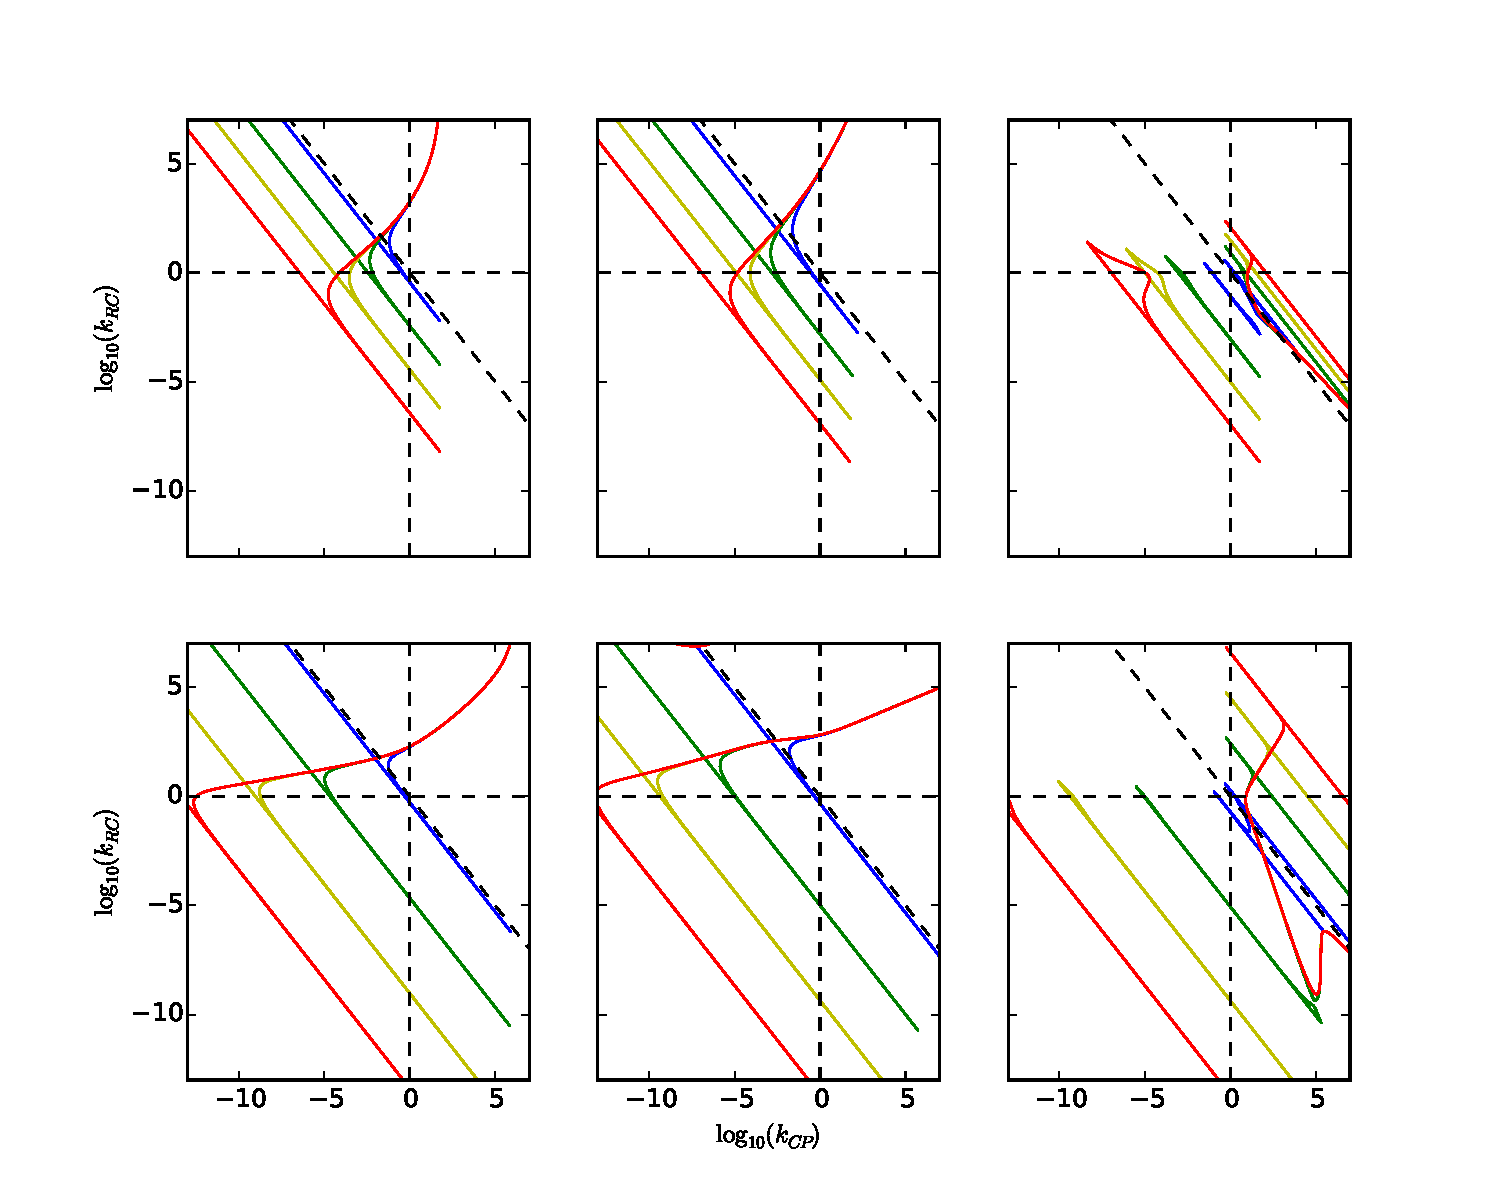
\includegraphics[width = 0.99\textwidth]{./Plots/Z(IC5)AcGrGr.pdf}
  \caption[Env $Z(IC5)$]{\emph{Envolturas de Invasibilidad} para el caso de el depredador intermedio $C$ como invasor frente a una comunidad receptora formada por $R-P$. Las dem\'as especificaciones se comparten con la figura ~\ref{fig:Z(IC2)}.}
  \label{fig:Z(IC5)}
\end{figure}



\subsubsection{\emph{Invasibilidad Mutua}}

La zona de invasi\'on mutua $Z_M$ al ser la interescci\'on de las dos zonas anteriores($Z_{\PP \to \R-\C}$ y $ Z_{\C \to \R-\PP}$, comparte principalmente con $Z(I_{\C \to \PP- \R})$ ,el patr\'on de variaci\'on respecto a cambios en $m_P$, $k_0$ y $\phi$. Adem\'as de ello su forma esta principalmente determinada por $Z(I_{\C \to \PP- \R})$\\
Para $\phi = 2$ y valores elevados de $m_p$ o $k_0$ posee dos componentes conexas, en este caso la diferencia entre $Z_M$ y $Z(I_{\C \to \PP- \R})$ se debe a variaciones en $\vartheta_C^1$ en ambientes de b\'usqueda $2D$ y en $\vartheta_C^2$ en el caso $3D$. Para $\phi = 0.02,0.2$ la diferencia se debe a la presencia de un borde superior el cual reduce la inclusi\'on de comunidades $C_2$ y $C_3$.\\
Adem\'as es notoria la reducci\'on en el \'area total de $Z_M$ con respecto a las anteriores.

\begin{figure}
  \centering
  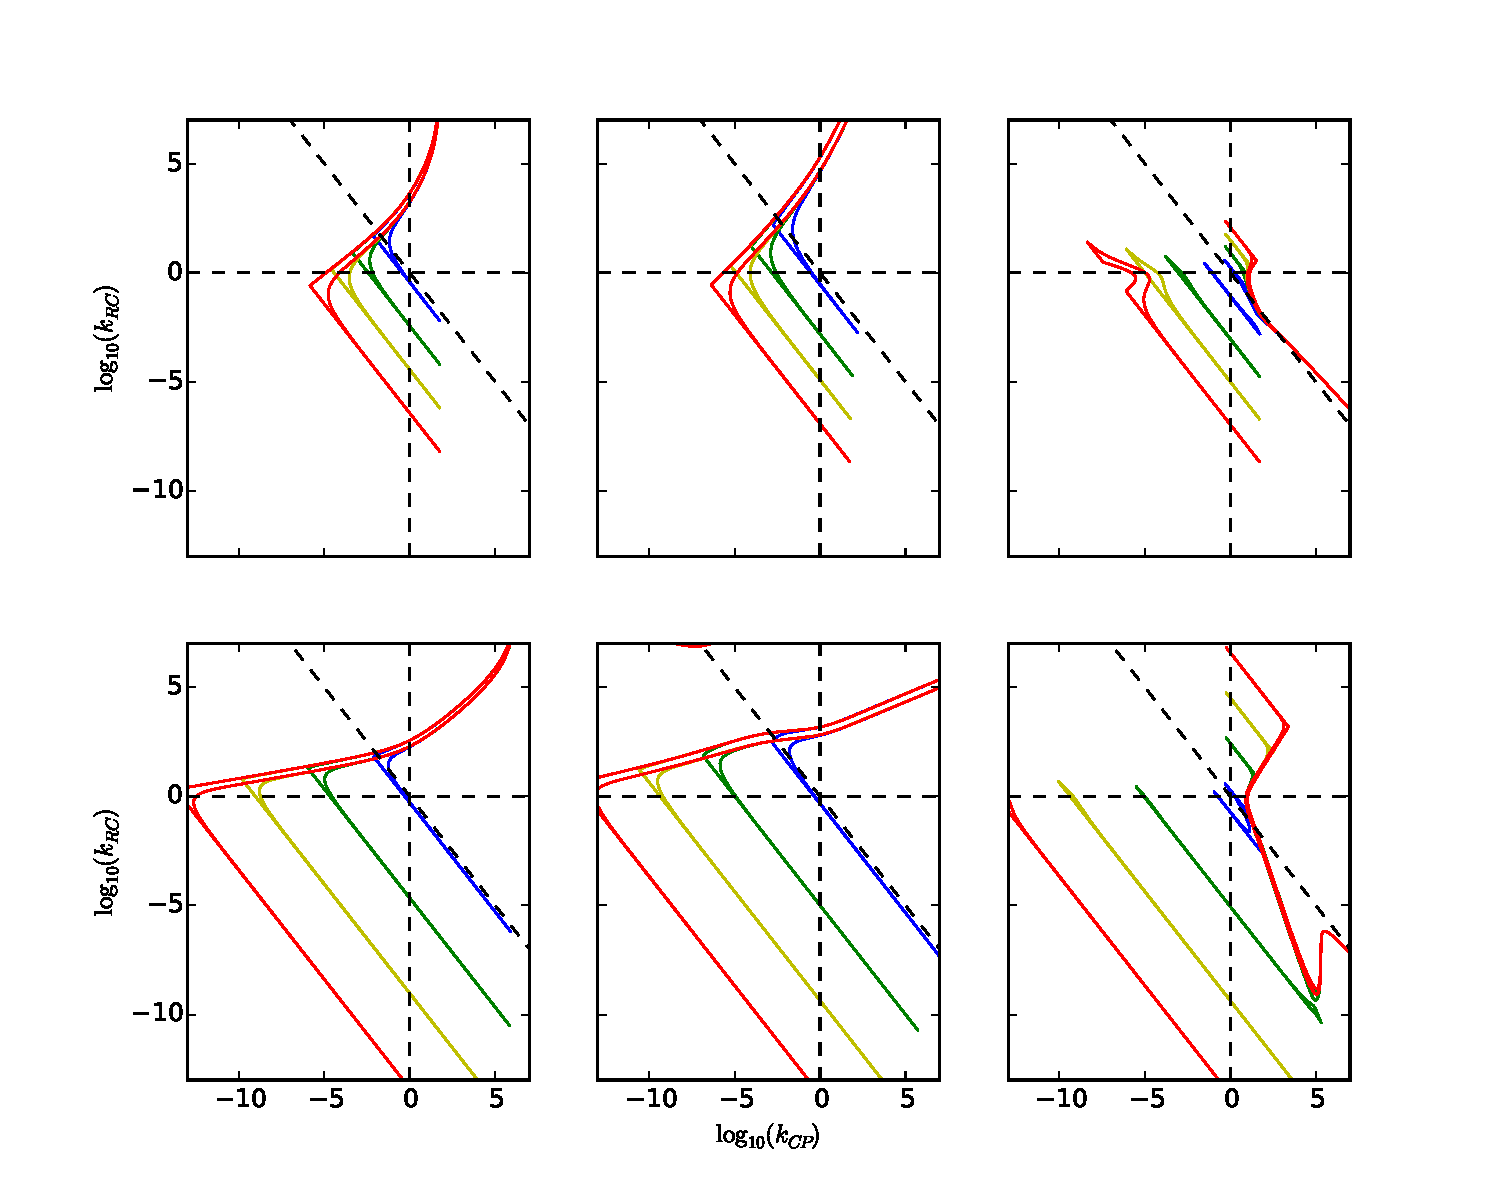
\includegraphics[width = 0.99\textwidth]{./Plots/MutualInvAcGrGr.pdf}
  \caption[Env $I_M$]{\emph{Envolturas de Invasibilidad Mutua} donde ambas sequencias de invasi\'on $S_1$ y $S_2$ dan lugar al m\'odulo completo. Las dem\'as especificaciones se comparten con la figura ~\ref{fig:Z(IC4)}.}
  \label{fig:MutualInv}
\end{figure}


En lo sucesivo nos referimos a la regi\'on $E_1$ dado que $E_2$ representa una parte muy peque\~na de $E$

\subsection{Coexistencia}

La regi\'on de coexistencia comparte el comportamiento cualitativo descrito para el caso de la zona de invasibilidad mutua, con su \'area total siendo afectada positivamente por $m_P$ y $k_0$ y $\phi$ afectando principalmente la conectividad de la zona, y generando para $\phi = 2$, dos subzonas diferenciadas principalmente por el valor de $k_{\RP}$ mayor o menor que 1 respectivamente.La distancia entre estas subzonas es afectada posivamente por $m_P$ y $k_0$. \\

A su vez la sub-regi\'on de coexistencia asociada a un equilibrio inestable se ve afectada por $m_P$($k_0$ afecta de manera similar) y $phi$ , donde tenemos que para la zona ``pico'' de inestabilidad(e.g alrededor de $k_{\RC} = 0$ para $m_P = 10^5$ y $\phi = 0.2$) la proporci\'on ocupada respecto a la region total de coexistencia aumenta con respecto a $m_p$ (v\'ease ~\ref{fig:CoexistenceWidth}) ,sin embargo dado que $m_P$ aumenta el \'area total de coexistencia,la proporci\'on inestable en general disminuye con $m_P$($k_0$). Para $\phi = 2$ tenemos que toda el \'area de coexistencia es estable.

\begin{figure}
  \centering
  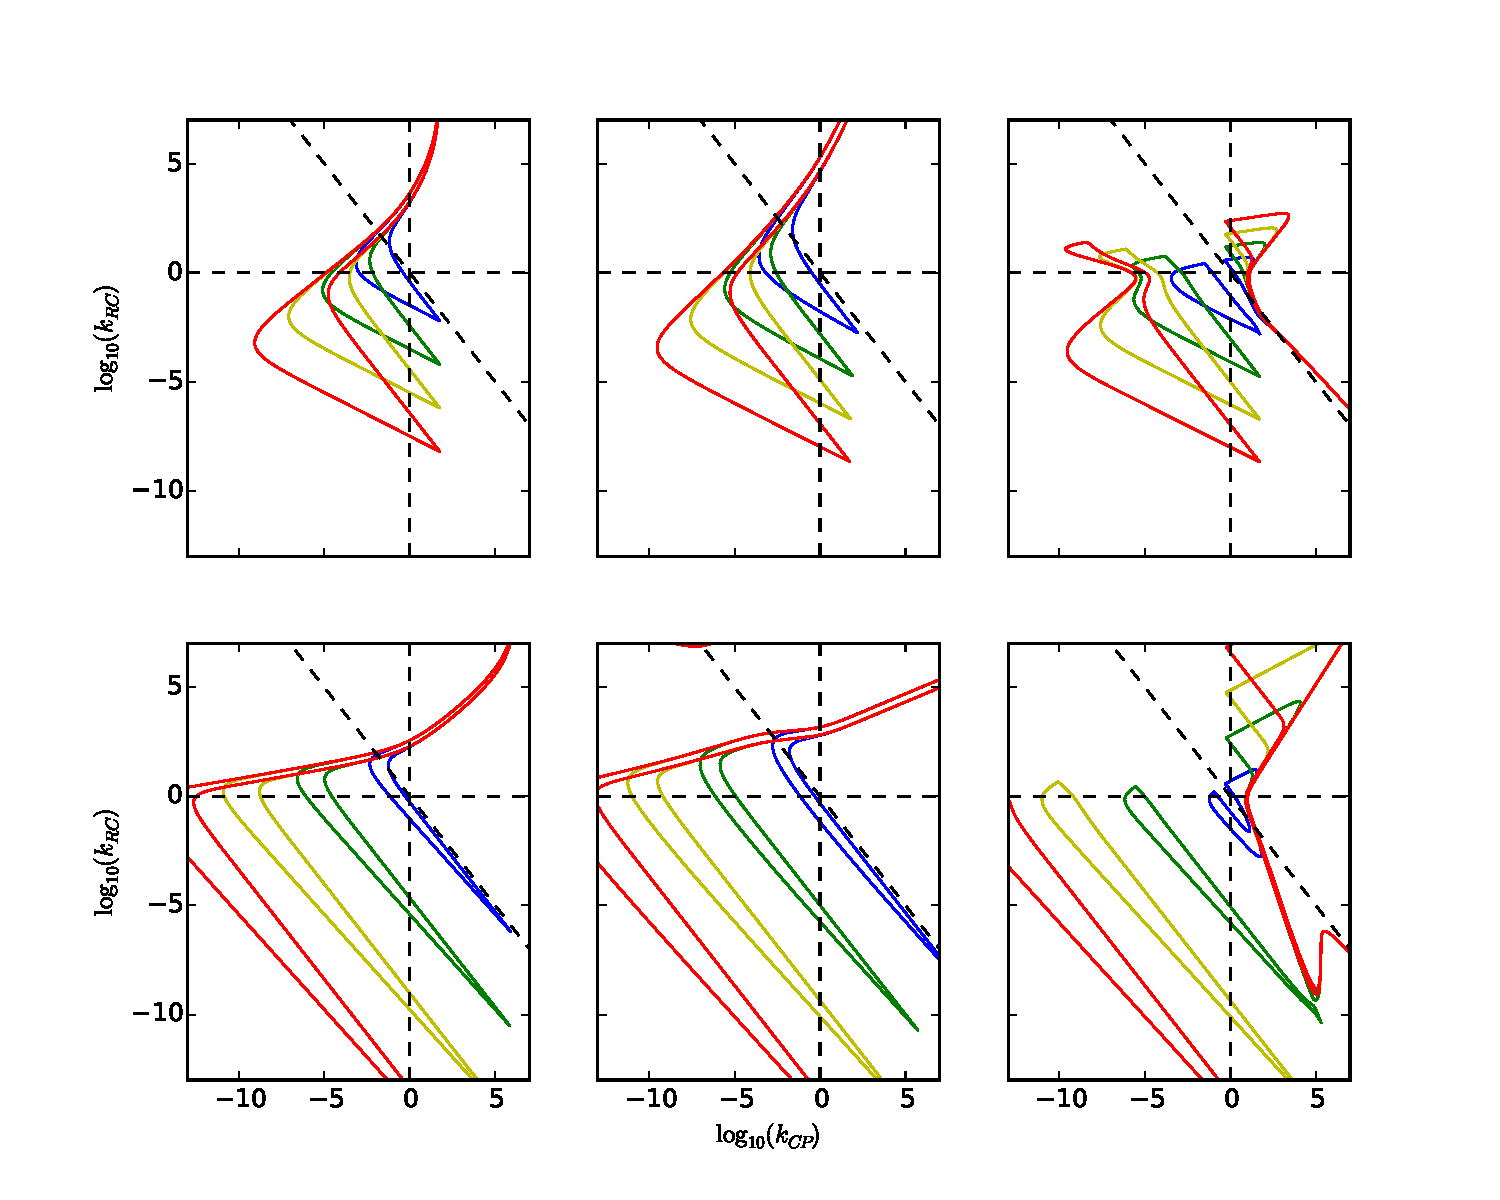
\includegraphics[width = 0.99\textwidth]{./Plots/CoexistenceAcGrGr.pdf}
  \caption[Env $Coexistencia$]{\emph{Coexistencia} donde existe un equilibrio $(R,C,P)$ positivo y este puede ser formado \emph{potencialmente} mediante una secuencia de ensamblaje($S_1$ o $S_2$. Las dem\'as especificaciones se comparten con la figura ~\ref{fig:Z(IC4)}.}
  \label{fig:PSCoexistence}
\end{figure}


\begin{figure}
  \centering
  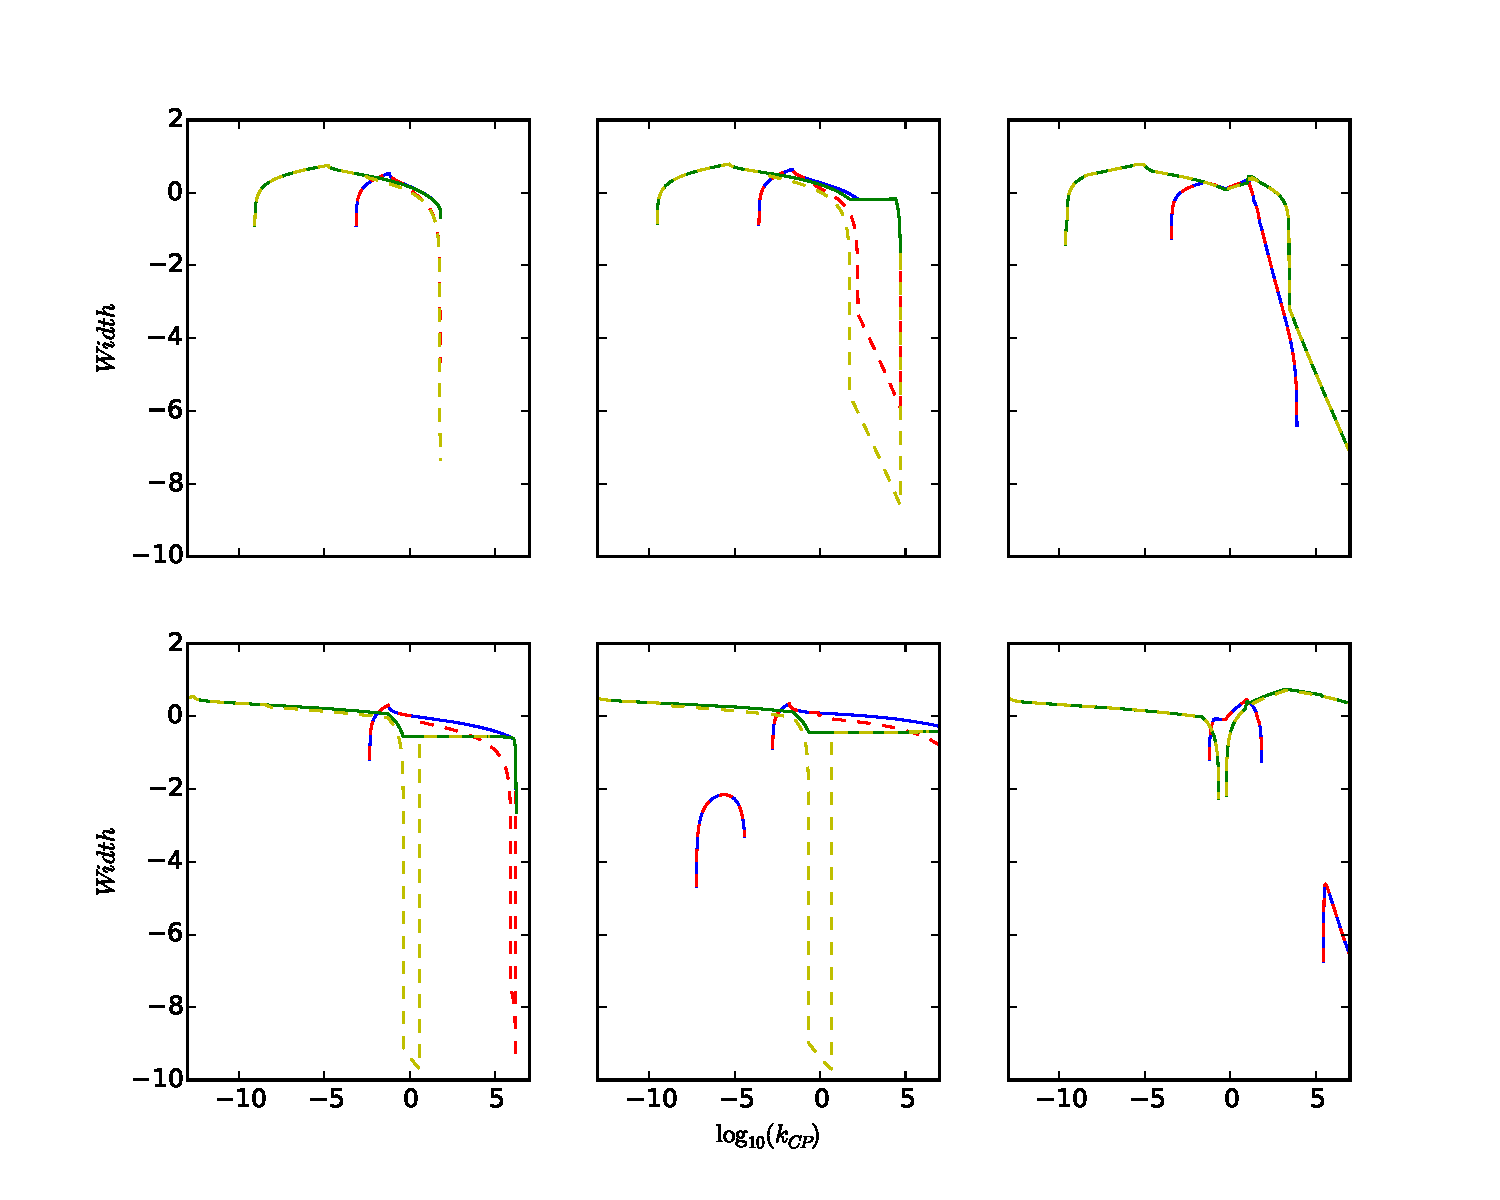
\includegraphics[width = 0.99\textwidth]{./Plots/WidthCoexistenceAcGrGr.pdf}
  \caption[Ancho $Coexistencia$]{Anchos de la zona de \emph{coexistencia} y la zona de \emph{coexistencia estable} respecto a cambios en los valores de $k_{\RC}$.({\hwplotT}) denota \emph{coexistencia} y ({\hwplotK}) \emph{coexistencia estable} . ({\hwplotG}) y  ({\hwplotY}) $10^5 kg$ , ({\hwplotR}) y ({\hwplotB}) para $10^{-10}kg$. Las dem\'as especificaciones se comparten con la figura ~\ref{fig:Z(IC4)}.}
  \label{fig:CoexistenceWidth}
\end{figure}























